\documentclass[twoside]{book}

% Packages required by doxygen
\usepackage{calc}
\usepackage{doxygen}
\usepackage{graphicx}
\usepackage[utf8]{inputenc}
\usepackage{makeidx}
\usepackage{multicol}
\usepackage{multirow}
\usepackage{textcomp}
\usepackage[table]{xcolor}

% NLS support packages
\usepackage[T2A]{fontenc}
\usepackage[russian]{babel}

% Font selection
\usepackage[T1]{fontenc}
\usepackage{mathptmx}
\usepackage[scaled=.90]{helvet}
\usepackage{courier}
\usepackage{amssymb}
\usepackage{sectsty}
\renewcommand{\familydefault}{\sfdefault}
\allsectionsfont{%
  \fontseries{bc}\selectfont%
  \color{darkgray}%
}
\renewcommand{\DoxyLabelFont}{%
  \fontseries{bc}\selectfont%
  \color{darkgray}%
}

% Page & text layout
\usepackage{geometry}
\geometry{%
  a4paper,%
  top=2.5cm,%
  bottom=2.5cm,%
  left=2.5cm,%
  right=2.5cm%
}
\tolerance=750
\hfuzz=15pt
\hbadness=750
\setlength{\emergencystretch}{15pt}
\setlength{\parindent}{0cm}
\setlength{\parskip}{0.2cm}
\makeatletter
\renewcommand{\paragraph}{%
  \@startsection{paragraph}{4}{0ex}{-1.0ex}{1.0ex}{%
    \normalfont\normalsize\bfseries\SS@parafont%
  }%
}
\renewcommand{\subparagraph}{%
  \@startsection{subparagraph}{5}{0ex}{-1.0ex}{1.0ex}{%
    \normalfont\normalsize\bfseries\SS@subparafont%
  }%
}
\makeatother

% Headers & footers
\usepackage{fancyhdr}
\pagestyle{fancyplain}
\fancyhead[LE]{\fancyplain{}{\bfseries\thepage}}
\fancyhead[CE]{\fancyplain{}{}}
\fancyhead[RE]{\fancyplain{}{\bfseries\leftmark}}
\fancyhead[LO]{\fancyplain{}{\bfseries\rightmark}}
\fancyhead[CO]{\fancyplain{}{}}
\fancyhead[RO]{\fancyplain{}{\bfseries\thepage}}
\fancyfoot[LE]{\fancyplain{}{}}
\fancyfoot[CE]{\fancyplain{}{}}
\fancyfoot[RE]{\fancyplain{}{\bfseries\scriptsize Документация по M\-P\-I Worker. Последние изменения\-: Ср 8 Июн 2016 18\-:12\-:00. Создано системой Doxygen }}
\fancyfoot[LO]{\fancyplain{}{\bfseries\scriptsize Документация по M\-P\-I Worker. Последние изменения\-: Ср 8 Июн 2016 18\-:12\-:00. Создано системой Doxygen }}
\fancyfoot[CO]{\fancyplain{}{}}
\fancyfoot[RO]{\fancyplain{}{}}
\renewcommand{\footrulewidth}{0.4pt}
\renewcommand{\chaptermark}[1]{%
  \markboth{#1}{}%
}
\renewcommand{\sectionmark}[1]{%
  \markright{\thesection\ #1}%
}

% Indices & bibliography
\usepackage{natbib}
\usepackage[titles]{tocloft}
\setcounter{tocdepth}{3}
\setcounter{secnumdepth}{5}
\makeindex

% Hyperlinks (required, but should be loaded last)
\usepackage{ifpdf}
\ifpdf
  \usepackage[pdftex,pagebackref=true]{hyperref}
\else
  \usepackage[ps2pdf,pagebackref=true]{hyperref}
\fi
\hypersetup{%
  colorlinks=true,%
  linkcolor=blue,%
  citecolor=blue,%
  unicode%
}

% Custom commands
\newcommand{\clearemptydoublepage}{%
  \newpage{\pagestyle{empty}\cleardoublepage}%
}


%===== C O N T E N T S =====

\begin{document}

% Titlepage & ToC
\hypersetup{pageanchor=false}
\pagenumbering{roman}
\begin{titlepage}
\vspace*{7cm}
\begin{center}%
{\Large M\-P\-I Worker }\\
\vspace*{1cm}
{\large Создано системой Doxygen 1.8.6}\\
\vspace*{0.5cm}
{\small Ср 8 Июн 2016 18:12:00}\\
\end{center}
\end{titlepage}
\clearemptydoublepage
\tableofcontents
\clearemptydoublepage
\pagenumbering{arabic}
\hypersetup{pageanchor=true}

%--- Begin generated contents ---
\chapter{Описание проекта}
\label{index}\hypertarget{index}{}\subsubsection*{Класс \hyperlink{classmpiworker_1_1MPIWorker}{mpiworker\-::\-M\-P\-I\-Worker}}

Содержит методы-\/обертки с простым синтаксисом для коллективных операций \href{https://www.open-mpi.org/}{\tt M\-P\-I} (Scatterv, Gatherv и других). Данные храняться в векторах \href{http://ru.cppreference.com/w/cpp/container/vector}{\tt std\-::vector}, работа выполняется в коммуникаторе M\-P\-I\-::\-C\-O\-M\-M\-\_\-\-W\-O\-R\-L\-D.

Для выполнения коллективных операций требуется создать объект класса M\-P\-I\-Worker\-: 
\begin{DoxyCode}
\hyperlink{classmpiworker_1_1MPIWorker}{mpiworker::MPIWorker} w;
\end{DoxyCode}
 затем установить режим работы и общее число обрабатываемых элементов 
\begin{DoxyCode}
w.\hyperlink{classmpiworker_1_1MPIWorker_a2ff88f266efae23ec2a12a56bd0472d1}{setMode}(0);
w.\hyperlink{classmpiworker_1_1MPIWorker_afcce321227c6d15a5fc2145cf59cd54d}{setNElems}(9999);
\end{DoxyCode}


Пример разделения элементов вектора на приблизительно равные части\-: 
\begin{DoxyCode}
\textcolor{comment}{// result for nNodes = 3}

  \hyperlink{classmpiworker_1_1MPIWorker}{mpiworker::MPIWorker} w;                          \textcolor{comment}{// MPI::Init(), Get\_size() and
       Get\_rank()}

  \textcolor{keywordtype}{int} N = 0; 
  std::vector<float> x; 

  \textcolor{keywordflow}{if}( !w.\hyperlink{classmpiworker_1_1MPIWorker_acbd3bd07d15ffa90a2c112edeecee6e0}{getRankNode}() ) 
  \{ 
      N = 11; 
      x.resize(N);
      std::iota(x.begin(),x.end(),1);              \textcolor{comment}{// rank=0: x = \{1, 2, 3, 4, 5, 6, 7, 8, 9, 10, 11\}}
  \}

  w.\hyperlink{classmpiworker_1_1MPIWorker_ae22bafa8bd4d6515e5b91ef95518c87d}{bcast}<\textcolor{keywordtype}{int}>(N,MPI::INT);                        \textcolor{comment}{// N == 11 on all ranks}
  w.\hyperlink{classmpiworker_1_1MPIWorker_a2ff88f266efae23ec2a12a56bd0472d1}{setMode}(1);                                    \textcolor{comment}{// all nodes have equal rights}
  w.\hyperlink{classmpiworker_1_1MPIWorker_afcce321227c6d15a5fc2145cf59cd54d}{setNElems}(N);                                  \textcolor{comment}{// counts = \{ 3, 4, 4 \}}
                                                   \textcolor{comment}{// displacement  = \{ 0, 3, 7 \}}
  \textcolor{keywordflow}{if}( !w.\hyperlink{classmpiworker_1_1MPIWorker_acbd3bd07d15ffa90a2c112edeecee6e0}{getRankNode}() ) w.\hyperlink{classmpiworker_1_1MPIWorker_ab9f20357773fe10fbe3bc6d92754d4e0}{print}();

  std::vector<float> xPerNode;                     \textcolor{comment}{// vector for local portions}
  w.\hyperlink{classmpiworker_1_1MPIWorker_a24f713941043ab8d54574830a251995b}{scatterv}<\textcolor{keywordtype}{float}>(x,xPerNode,MPI::FLOAT);        \textcolor{comment}{// rank=0: \{ 1, 2, 3 \}}
                                                   \textcolor{comment}{// rank=1: \{ 4, 5, 6, 7 \}}
                                                   \textcolor{comment}{// rank=2: \{ 8, 9, 10, 11 \}}
  \textcolor{keywordflow}{for}( \textcolor{keyword}{auto} & e: xPerNode)
  \{
      e += w.\hyperlink{classmpiworker_1_1MPIWorker_acbd3bd07d15ffa90a2c112edeecee6e0}{getRankNode}();                        \textcolor{comment}{// rank=0: \{ 1, 2, 3 \}}
  \}                                                \textcolor{comment}{// rank=1: \{ 5, 6, 7, 8 \}}
                                                   \textcolor{comment}{// rank=2: \{ 10, 11, 12, 13 \}}
  std::vector<float> y( N );
  w.\hyperlink{classmpiworker_1_1MPIWorker_aff6b4d55cb55caa37c9a0cb08b3c5661}{gatherv}( xPerNode, y, MPI::FLOAT );            \textcolor{comment}{// rank=0: \{ 1, 2, 3, 5, 6, 7, 8, 10, 11, 12, 13
       \}}
                                                   \textcolor{comment}{// rank=1,2: \{ 0, 0, 0, 0, 0, 0, 0, 0, 0, 0, 0 \}}

  w.\hyperlink{classmpiworker_1_1MPIWorker_a49fda2aa379265e74f9b7504ad67ee9a}{allGatherv}( xPerNode, y, MPI::FLOAT );         \textcolor{comment}{// rank=0,1,2: \{ 1, 2, 3, 5, 6, 7, 8, 10, 11,
       12, 13 \}}
\end{DoxyCode}


Класс \hyperlink{classmpiworker_1_1MPIInit}{mpiworker\-::\-M\-P\-I\-Init} и функция calculate\-Portions играют вспомогательную роль, но могут быть использованы независимо от \hyperlink{classmpiworker_1_1MPIWorker}{mpiworker\-::\-M\-P\-I\-Worker}.

\subsubsection*{Класс \hyperlink{classmpiworker_1_1MPIInit}{mpiworker\-::\-M\-P\-I\-Init}}

Выполняет инициализацию и закрытие библиотеки M\-P\-I. Реализован как Singleton Meyers.

\subsubsection*{Функция \href{group__MPIWorker.html#ga6fd8303c1b4e39a4a623756fdcbeae6f}{\tt calculate\-Portions}}

Выполняет формирование вспомогательных массивов для деления некоторого общего количества элементов на приблизительно равные части коллективной операцией Scatterv или для объединения массивов значений на узлах в единый массив. 
\chapter{Алфавитный указатель групп}
\section{Группы}
Полный список групп.\begin{DoxyCompactList}
\item \contentsline{section}{M\-P\-I\-Worker}{\pageref{group__MPIWorker}}{}
\end{DoxyCompactList}

\chapter{Алфавитный указатель пространств имен}
\section{Namespace List}
Here is a list of all namespaces with brief descriptions\-:\begin{DoxyCompactList}
\item\contentsline{section}{\hyperlink{namespacempiworker}{mpiworker} }{\pageref{namespacempiworker}}{}
\end{DoxyCompactList}

\chapter{Алфавитный указатель классов}
\section{Class List}
Here are the classes, structs, unions and interfaces with brief descriptions\-:\begin{DoxyCompactList}
\item\contentsline{section}{\hyperlink{classmpiworker_1_1MPIInit}{mpiworker\-::\-M\-P\-I\-Init} }{\pageref{classmpiworker_1_1MPIInit}}{}
\item\contentsline{section}{\hyperlink{classmpiworker_1_1MPIWorker}{mpiworker\-::\-M\-P\-I\-Worker} }{\pageref{classmpiworker_1_1MPIWorker}}{}
\end{DoxyCompactList}

\chapter{Список файлов}
\section{File List}
Here is a list of all files with brief descriptions\-:\begin{DoxyCompactList}
\item\contentsline{section}{\hyperlink{mpiworker_8hpp}{mpiworker.\-hpp} }{\pageref{mpiworker_8hpp}}{}
\item\contentsline{section}{\hyperlink{test__scatter__then__gather_8cpp}{test\-\_\-scatter\-\_\-then\-\_\-gather.\-cpp} }{\pageref{test__scatter__then__gather_8cpp}}{}
\item\contentsline{section}{\hyperlink{tools__for__parallel_8hpp}{tools\-\_\-for\-\_\-parallel.\-hpp} }{\pageref{tools__for__parallel_8hpp}}{}
\end{DoxyCompactList}

\chapter{Группы}
\hypertarget{group__MPIWorker}{\section{M\-P\-I\-Worker}
\label{group__MPIWorker}\index{M\-P\-I\-Worker@{M\-P\-I\-Worker}}
}
\subsection*{Файлы}
\begin{DoxyCompactItemize}
\item 
файл \hyperlink{mpiworker_8hpp}{mpiworker.\-hpp}
\item 
файл \hyperlink{tools__for__parallel_8hpp}{tools\-\_\-for\-\_\-parallel.\-hpp}
\end{DoxyCompactItemize}
\subsection*{Пространства имен}
\begin{DoxyCompactItemize}
\item 
\hyperlink{namespacempiworker}{mpiworker}
\end{DoxyCompactItemize}
\subsection*{Функции}
\begin{DoxyCompactItemize}
\item 
{\footnotesize template$<$typename Iterator , typename Size\-Type $>$ }\\void \hyperlink{group__MPIWorker_ga6fd8303c1b4e39a4a623756fdcbeae6f}{calculate\-Portions} (Size\-Type n\-Elems, Iterator beg\-Counts, Iterator end\-Counts, Iterator beg\-Displs, Iterator end\-Displs, bool is\-Zero\-Work=false)
\begin{DoxyCompactList}\small\item\em Функция выполняет разделение элементов на приблизительно одинаковые порции. Формирует вспомагательные массивы для M\-P\-I функций M\-P\-I\-\_\-\-Gatherv and M\-P\-I\-\_\-\-Scatterv. Поддерживает схемы\-: \end{DoxyCompactList}\end{DoxyCompactItemize}


\subsection{Подробное описание}


\subsection{Функции}
\hypertarget{group__MPIWorker_ga6fd8303c1b4e39a4a623756fdcbeae6f}{\index{M\-P\-I\-Worker@{M\-P\-I\-Worker}!calculate\-Portions@{calculate\-Portions}}
\index{calculate\-Portions@{calculate\-Portions}!MPIWorker@{M\-P\-I\-Worker}}
\subsubsection[{calculate\-Portions}]{\setlength{\rightskip}{0pt plus 5cm}template$<$typename Iterator , typename Size\-Type $>$ void calculate\-Portions (
\begin{DoxyParamCaption}
\item[{Size\-Type}]{n\-Elems, }
\item[{Iterator}]{beg\-Counts, }
\item[{Iterator}]{end\-Counts, }
\item[{Iterator}]{beg\-Displs, }
\item[{Iterator}]{end\-Displs, }
\item[{bool}]{is\-Zero\-Work = {\ttfamily false}}
\end{DoxyParamCaption}
)}}\label{group__MPIWorker_ga6fd8303c1b4e39a4a623756fdcbeae6f}


Функция выполняет разделение элементов на приблизительно одинаковые порции. Формирует вспомагательные массивы для M\-P\-I функций M\-P\-I\-\_\-\-Gatherv and M\-P\-I\-\_\-\-Scatterv. Поддерживает схемы\-: 


\begin{DoxyItemize}
\item с управляющим нулевым узлом;
\item все узлы равноправны. 
\end{DoxyItemize}
\begin{DoxyParams}{Аргументы}
{\em n\-Elems} & Число элементов \\
\hline
\end{DoxyParams}

\chapter{Пространства имен}
\hypertarget{namespacempiworker}{\section{mpiworker Namespace Reference}
\label{namespacempiworker}\index{mpiworker@{mpiworker}}
}
\subsection*{Classes}
\begin{DoxyCompactItemize}
\item 
class \hyperlink{classmpiworker_1_1MPIInit}{M\-P\-I\-Init}
\item 
class \hyperlink{classmpiworker_1_1MPIWorker}{M\-P\-I\-Worker}
\end{DoxyCompactItemize}

\chapter{Классы}
\hypertarget{classmpiworker_1_1MPIInit}{\section{Класс mpiworker\-:\-:M\-P\-I\-Init}
\label{classmpiworker_1_1MPIInit}\index{mpiworker\-::\-M\-P\-I\-Init@{mpiworker\-::\-M\-P\-I\-Init}}
}


Создает и удаляет коммуникатор M\-P\-I\-::\-C\-O\-M\-M\-\_\-\-W\-O\-R\-L\-D. Реализован как Singleton Meyers. Начиная с С++11 потокобезобасен \mbox{[}I\-S\-O N3337, 6.\-7.\-4\mbox{]}.  




{\ttfamily \#include $<$mpiworker.\-hpp$>$}



Граф связей класса mpiworker\-:\-:M\-P\-I\-Init\-:\nopagebreak
\begin{figure}[H]
\begin{center}
\leavevmode
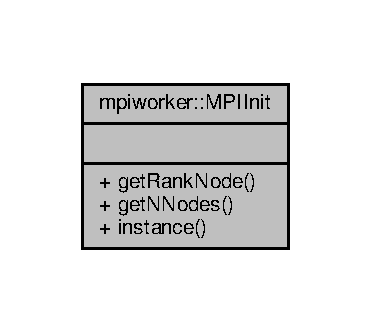
\includegraphics[width=178pt]{classmpiworker_1_1MPIInit__coll__graph}
\end{center}
\end{figure}
\subsection*{Открытые члены}
\begin{DoxyCompactItemize}
\item 
int \hyperlink{classmpiworker_1_1MPIInit_a9b44428732f6317268da287d1844d1c9}{get\-Rank\-Node} () const 
\begin{DoxyCompactList}\small\item\em Возвращает ранг узла. \end{DoxyCompactList}\item 
int \hyperlink{classmpiworker_1_1MPIInit_a7b8323075afa7a6d36015e66286183fc}{get\-N\-Nodes} () const 
\begin{DoxyCompactList}\small\item\em Возвращает число узлов. \end{DoxyCompactList}\end{DoxyCompactItemize}
\subsection*{Открытые статические члены}
\begin{DoxyCompactItemize}
\item 
static \hyperlink{classmpiworker_1_1MPIInit}{M\-P\-I\-Init} \& \hyperlink{classmpiworker_1_1MPIInit_a20d2436672af2589cb72200396a8aed6}{instance} ()
\end{DoxyCompactItemize}


\subsection{Подробное описание}
Создает и удаляет коммуникатор M\-P\-I\-::\-C\-O\-M\-M\-\_\-\-W\-O\-R\-L\-D. Реализован как Singleton Meyers. Начиная с С++11 потокобезобасен \mbox{[}I\-S\-O N3337, 6.\-7.\-4\mbox{]}. 

\subsection{Методы}
\hypertarget{classmpiworker_1_1MPIInit_a7b8323075afa7a6d36015e66286183fc}{\index{mpiworker\-::\-M\-P\-I\-Init@{mpiworker\-::\-M\-P\-I\-Init}!get\-N\-Nodes@{get\-N\-Nodes}}
\index{get\-N\-Nodes@{get\-N\-Nodes}!mpiworker::MPIInit@{mpiworker\-::\-M\-P\-I\-Init}}
\subsubsection[{get\-N\-Nodes}]{\setlength{\rightskip}{0pt plus 5cm}int mpiworker\-::\-M\-P\-I\-Init\-::get\-N\-Nodes (
\begin{DoxyParamCaption}
{}
\end{DoxyParamCaption}
) const\hspace{0.3cm}{\ttfamily [inline]}}}\label{classmpiworker_1_1MPIInit_a7b8323075afa7a6d36015e66286183fc}


Возвращает число узлов. 

\hypertarget{classmpiworker_1_1MPIInit_a9b44428732f6317268da287d1844d1c9}{\index{mpiworker\-::\-M\-P\-I\-Init@{mpiworker\-::\-M\-P\-I\-Init}!get\-Rank\-Node@{get\-Rank\-Node}}
\index{get\-Rank\-Node@{get\-Rank\-Node}!mpiworker::MPIInit@{mpiworker\-::\-M\-P\-I\-Init}}
\subsubsection[{get\-Rank\-Node}]{\setlength{\rightskip}{0pt plus 5cm}int mpiworker\-::\-M\-P\-I\-Init\-::get\-Rank\-Node (
\begin{DoxyParamCaption}
{}
\end{DoxyParamCaption}
) const\hspace{0.3cm}{\ttfamily [inline]}}}\label{classmpiworker_1_1MPIInit_a9b44428732f6317268da287d1844d1c9}


Возвращает ранг узла. 

\hypertarget{classmpiworker_1_1MPIInit_a20d2436672af2589cb72200396a8aed6}{\index{mpiworker\-::\-M\-P\-I\-Init@{mpiworker\-::\-M\-P\-I\-Init}!instance@{instance}}
\index{instance@{instance}!mpiworker::MPIInit@{mpiworker\-::\-M\-P\-I\-Init}}
\subsubsection[{instance}]{\setlength{\rightskip}{0pt plus 5cm}static {\bf M\-P\-I\-Init}\& mpiworker\-::\-M\-P\-I\-Init\-::instance (
\begin{DoxyParamCaption}
{}
\end{DoxyParamCaption}
)\hspace{0.3cm}{\ttfamily [inline]}, {\ttfamily [static]}}}\label{classmpiworker_1_1MPIInit_a20d2436672af2589cb72200396a8aed6}


Объявления и описания членов класса находятся в файле\-:\begin{DoxyCompactItemize}
\item 
\hyperlink{mpiworker_8hpp}{mpiworker.\-hpp}\end{DoxyCompactItemize}

\hypertarget{classmpiworker_1_1MPIWorker}{\section{Класс mpiworker\-:\-:M\-P\-I\-Worker}
\label{classmpiworker_1_1MPIWorker}\index{mpiworker\-::\-M\-P\-I\-Worker@{mpiworker\-::\-M\-P\-I\-Worker}}
}


Содержит методы, выполняющие разделение и сборку массивов в M\-P\-I-\/приложении.  




{\ttfamily \#include $<$mpiworker.\-hpp$>$}



Граф связей класса mpiworker\-:\-:M\-P\-I\-Worker\-:\nopagebreak
\begin{figure}[H]
\begin{center}
\leavevmode
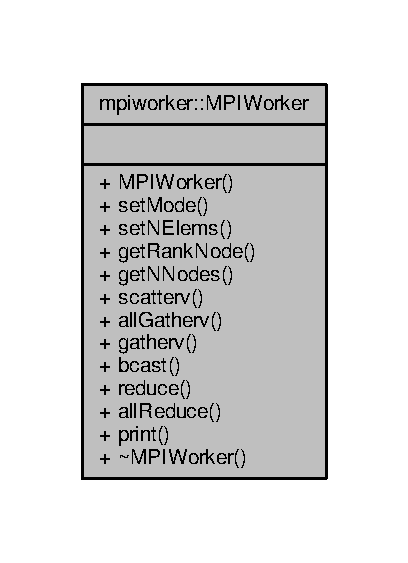
\includegraphics[width=196pt]{classmpiworker_1_1MPIWorker__coll__graph}
\end{center}
\end{figure}
\subsection*{Открытые члены}
\begin{DoxyCompactItemize}
\item 
\hyperlink{classmpiworker_1_1MPIWorker_a4c6b9d1a46edd8a52cf750974975cbea}{M\-P\-I\-Worker} ()
\begin{DoxyCompactList}\small\item\em Конструктор. \end{DoxyCompactList}\item 
void \hyperlink{classmpiworker_1_1MPIWorker_a2ff88f266efae23ec2a12a56bd0472d1}{set\-Mode} (const short \&mode)
\item 
void \hyperlink{classmpiworker_1_1MPIWorker_afcce321227c6d15a5fc2145cf59cd54d}{set\-N\-Elems} (const int \&n\-Elems)
\begin{DoxyCompactList}\small\item\em Число элементов в разрезаемом или собираемом массиве. \end{DoxyCompactList}\item 
int \hyperlink{classmpiworker_1_1MPIWorker_acbd3bd07d15ffa90a2c112edeecee6e0}{get\-Rank\-Node} () const 
\begin{DoxyCompactList}\small\item\em Возвращает ранг узла. \end{DoxyCompactList}\item 
int \hyperlink{classmpiworker_1_1MPIWorker_aeeb08c56600799093b3b9da60d337896}{get\-N\-Nodes} () const 
\begin{DoxyCompactList}\small\item\em Возвращает число узлов. \end{DoxyCompactList}\item 
{\footnotesize template$<$typename T $>$ }\\void \hyperlink{classmpiworker_1_1MPIWorker_a24f713941043ab8d54574830a251995b}{scatterv} (const std\-::vector$<$ T $>$ \&array, std\-::vector$<$ T $>$ \&array\-Per\-Node, M\-P\-I\-::\-Datatype M\-P\-I\-Type, bool is\-Resize=true)
\begin{DoxyCompactList}\small\item\em Разделение элементов массива на приблизительно равные части. \end{DoxyCompactList}\item 
{\footnotesize template$<$typename T $>$ }\\void \hyperlink{classmpiworker_1_1MPIWorker_a49fda2aa379265e74f9b7504ad67ee9a}{all\-Gatherv} (const std\-::vector$<$ T $>$ \&array\-Per\-Node, std\-::vector$<$ T $>$ \&array, M\-P\-I\-::\-Datatype M\-P\-I\-Type)
\begin{DoxyCompactList}\small\item\em Сбор элементов в единые массивы на всех узлах. \end{DoxyCompactList}\item 
{\footnotesize template$<$typename T $>$ }\\void \hyperlink{classmpiworker_1_1MPIWorker_aff6b4d55cb55caa37c9a0cb08b3c5661}{gatherv} (const std\-::vector$<$ T $>$ \&array\-Per\-Node, std\-::vector$<$ T $>$ \&array, M\-P\-I\-::\-Datatype M\-P\-I\-Type)
\begin{DoxyCompactList}\small\item\em Сбор элементов в единый массив на нулевом узле. \end{DoxyCompactList}\item 
{\footnotesize template$<$typename T $>$ }\\void \hyperlink{classmpiworker_1_1MPIWorker_ae22bafa8bd4d6515e5b91ef95518c87d}{bcast} (T \&var, M\-P\-I\-::\-Datatype M\-P\-I\-Type)
\begin{DoxyCompactList}\small\item\em Рассылает значение скалярной переменной с нулевого узла на все остальные. \end{DoxyCompactList}\item 
{\footnotesize template$<$typename T $>$ }\\void \hyperlink{classmpiworker_1_1MPIWorker_a813f812267563ac5000fdee9393ddfff}{reduce} (const std\-::vector$<$ T $>$ \&array\-Part, std\-::vector$<$ T $>$ \&array\-Res, M\-P\-I\-::\-Datatype M\-P\-I\-Type, M\-P\-I\-::\-Op M\-P\-I\-Op)
\begin{DoxyCompactList}\small\item\em Выполняет редукцию со сбором результата на нулевом узле \end{DoxyCompactList}\item 
{\footnotesize template$<$typename T $>$ }\\void \hyperlink{classmpiworker_1_1MPIWorker_ac612f81da30253de9e6c9fbc8eda7427}{all\-Reduce} (const std\-::vector$<$ T $>$ \&array\-Part, std\-::vector$<$ T $>$ \&array\-Res, M\-P\-I\-::\-Datatype M\-P\-I\-Type, M\-P\-I\-::\-Op M\-P\-I\-Op)
\begin{DoxyCompactList}\small\item\em Выполняет редукцию с сохранением результата на всех узлах \end{DoxyCompactList}\item 
void \hyperlink{classmpiworker_1_1MPIWorker_ab9f20357773fe10fbe3bc6d92754d4e0}{print} ()
\begin{DoxyCompactList}\small\item\em Печать значений, хранимых в полях. \end{DoxyCompactList}\item 
\hyperlink{classmpiworker_1_1MPIWorker_aed998fa1c473d6bc98150bb94dd8bb58}{$\sim$\-M\-P\-I\-Worker} ()
\begin{DoxyCompactList}\small\item\em Деструктор. \end{DoxyCompactList}\end{DoxyCompactItemize}


\subsection{Подробное описание}
Содержит методы, выполняющие разделение и сборку массивов в M\-P\-I-\/приложении. 

Методы класса представляют собой обертку к коллективным M\-P\-I-\/функциям Scatterv и Allgatherv. Работа выполняется в коммуникаторе C\-O\-M\-M\-\_\-\-W\-O\-R\-L\-D. Реализованы схемы\-:
\begin{DoxyItemize}
\item с управляющим нулевым узлом при set\-Mode(0);
\item все узлы выполняют вычисления при set\-Mode(1). 
\end{DoxyItemize}

\subsection{Конструктор(ы)}
\hypertarget{classmpiworker_1_1MPIWorker_a4c6b9d1a46edd8a52cf750974975cbea}{\index{mpiworker\-::\-M\-P\-I\-Worker@{mpiworker\-::\-M\-P\-I\-Worker}!M\-P\-I\-Worker@{M\-P\-I\-Worker}}
\index{M\-P\-I\-Worker@{M\-P\-I\-Worker}!mpiworker::MPIWorker@{mpiworker\-::\-M\-P\-I\-Worker}}
\subsubsection[{M\-P\-I\-Worker}]{\setlength{\rightskip}{0pt plus 5cm}mpiworker\-::\-M\-P\-I\-Worker\-::\-M\-P\-I\-Worker (
\begin{DoxyParamCaption}
{}
\end{DoxyParamCaption}
)\hspace{0.3cm}{\ttfamily [inline]}}}\label{classmpiworker_1_1MPIWorker_a4c6b9d1a46edd8a52cf750974975cbea}


Конструктор. 

\hypertarget{classmpiworker_1_1MPIWorker_aed998fa1c473d6bc98150bb94dd8bb58}{\index{mpiworker\-::\-M\-P\-I\-Worker@{mpiworker\-::\-M\-P\-I\-Worker}!$\sim$\-M\-P\-I\-Worker@{$\sim$\-M\-P\-I\-Worker}}
\index{$\sim$\-M\-P\-I\-Worker@{$\sim$\-M\-P\-I\-Worker}!mpiworker::MPIWorker@{mpiworker\-::\-M\-P\-I\-Worker}}
\subsubsection[{$\sim$\-M\-P\-I\-Worker}]{\setlength{\rightskip}{0pt plus 5cm}mpiworker\-::\-M\-P\-I\-Worker\-::$\sim$\-M\-P\-I\-Worker (
\begin{DoxyParamCaption}
{}
\end{DoxyParamCaption}
)\hspace{0.3cm}{\ttfamily [inline]}}}\label{classmpiworker_1_1MPIWorker_aed998fa1c473d6bc98150bb94dd8bb58}


Деструктор. 



\subsection{Методы}
\hypertarget{classmpiworker_1_1MPIWorker_a49fda2aa379265e74f9b7504ad67ee9a}{\index{mpiworker\-::\-M\-P\-I\-Worker@{mpiworker\-::\-M\-P\-I\-Worker}!all\-Gatherv@{all\-Gatherv}}
\index{all\-Gatherv@{all\-Gatherv}!mpiworker::MPIWorker@{mpiworker\-::\-M\-P\-I\-Worker}}
\subsubsection[{all\-Gatherv}]{\setlength{\rightskip}{0pt plus 5cm}template$<$typename T $>$ void mpiworker\-::\-M\-P\-I\-Worker\-::all\-Gatherv (
\begin{DoxyParamCaption}
\item[{const std\-::vector$<$ T $>$ \&}]{array\-Per\-Node, }
\item[{std\-::vector$<$ T $>$ \&}]{array, }
\item[{M\-P\-I\-::\-Datatype}]{M\-P\-I\-Type}
\end{DoxyParamCaption}
)\hspace{0.3cm}{\ttfamily [inline]}}}\label{classmpiworker_1_1MPIWorker_a49fda2aa379265e74f9b7504ad67ee9a}


Сбор элементов в единые массивы на всех узлах. 


\begin{DoxyParams}[1]{Аргументы}
\mbox{\tt in}  & {\em array\-Per\-Node} & Входной массив с элементами текущего узла. \\
\hline
\mbox{\tt out}  & {\em array} & Итоговый массив со всеми элементами. \\
\hline
\mbox{\tt in}  & {\em M\-P\-I\-Type} & Тип элементов. \\
\hline
\end{DoxyParams}
\hypertarget{classmpiworker_1_1MPIWorker_ac612f81da30253de9e6c9fbc8eda7427}{\index{mpiworker\-::\-M\-P\-I\-Worker@{mpiworker\-::\-M\-P\-I\-Worker}!all\-Reduce@{all\-Reduce}}
\index{all\-Reduce@{all\-Reduce}!mpiworker::MPIWorker@{mpiworker\-::\-M\-P\-I\-Worker}}
\subsubsection[{all\-Reduce}]{\setlength{\rightskip}{0pt plus 5cm}template$<$typename T $>$ void mpiworker\-::\-M\-P\-I\-Worker\-::all\-Reduce (
\begin{DoxyParamCaption}
\item[{const std\-::vector$<$ T $>$ \&}]{array\-Part, }
\item[{std\-::vector$<$ T $>$ \&}]{array\-Res, }
\item[{M\-P\-I\-::\-Datatype}]{M\-P\-I\-Type, }
\item[{M\-P\-I\-::\-Op}]{M\-P\-I\-Op}
\end{DoxyParamCaption}
)\hspace{0.3cm}{\ttfamily [inline]}}}\label{classmpiworker_1_1MPIWorker_ac612f81da30253de9e6c9fbc8eda7427}


Выполняет редукцию с сохранением результата на всех узлах 

\hypertarget{classmpiworker_1_1MPIWorker_ae22bafa8bd4d6515e5b91ef95518c87d}{\index{mpiworker\-::\-M\-P\-I\-Worker@{mpiworker\-::\-M\-P\-I\-Worker}!bcast@{bcast}}
\index{bcast@{bcast}!mpiworker::MPIWorker@{mpiworker\-::\-M\-P\-I\-Worker}}
\subsubsection[{bcast}]{\setlength{\rightskip}{0pt plus 5cm}template$<$typename T $>$ void mpiworker\-::\-M\-P\-I\-Worker\-::bcast (
\begin{DoxyParamCaption}
\item[{T \&}]{var, }
\item[{M\-P\-I\-::\-Datatype}]{M\-P\-I\-Type}
\end{DoxyParamCaption}
)\hspace{0.3cm}{\ttfamily [inline]}}}\label{classmpiworker_1_1MPIWorker_ae22bafa8bd4d6515e5b91ef95518c87d}


Рассылает значение скалярной переменной с нулевого узла на все остальные. 

\hypertarget{classmpiworker_1_1MPIWorker_aff6b4d55cb55caa37c9a0cb08b3c5661}{\index{mpiworker\-::\-M\-P\-I\-Worker@{mpiworker\-::\-M\-P\-I\-Worker}!gatherv@{gatherv}}
\index{gatherv@{gatherv}!mpiworker::MPIWorker@{mpiworker\-::\-M\-P\-I\-Worker}}
\subsubsection[{gatherv}]{\setlength{\rightskip}{0pt plus 5cm}template$<$typename T $>$ void mpiworker\-::\-M\-P\-I\-Worker\-::gatherv (
\begin{DoxyParamCaption}
\item[{const std\-::vector$<$ T $>$ \&}]{array\-Per\-Node, }
\item[{std\-::vector$<$ T $>$ \&}]{array, }
\item[{M\-P\-I\-::\-Datatype}]{M\-P\-I\-Type}
\end{DoxyParamCaption}
)\hspace{0.3cm}{\ttfamily [inline]}}}\label{classmpiworker_1_1MPIWorker_aff6b4d55cb55caa37c9a0cb08b3c5661}


Сбор элементов в единый массив на нулевом узле. 


\begin{DoxyParams}[1]{Аргументы}
\mbox{\tt in}  & {\em array\-Per\-Node} & Входной массив с элементами текущего узла. \\
\hline
\mbox{\tt out}  & {\em array} & Итоговый массив со всеми элементами. \\
\hline
\mbox{\tt in}  & {\em M\-P\-I\-Type} & Тип элементов. \\
\hline
\end{DoxyParams}
\hypertarget{classmpiworker_1_1MPIWorker_aeeb08c56600799093b3b9da60d337896}{\index{mpiworker\-::\-M\-P\-I\-Worker@{mpiworker\-::\-M\-P\-I\-Worker}!get\-N\-Nodes@{get\-N\-Nodes}}
\index{get\-N\-Nodes@{get\-N\-Nodes}!mpiworker::MPIWorker@{mpiworker\-::\-M\-P\-I\-Worker}}
\subsubsection[{get\-N\-Nodes}]{\setlength{\rightskip}{0pt plus 5cm}int mpiworker\-::\-M\-P\-I\-Worker\-::get\-N\-Nodes (
\begin{DoxyParamCaption}
{}
\end{DoxyParamCaption}
) const\hspace{0.3cm}{\ttfamily [inline]}}}\label{classmpiworker_1_1MPIWorker_aeeb08c56600799093b3b9da60d337896}


Возвращает число узлов. 

\hypertarget{classmpiworker_1_1MPIWorker_acbd3bd07d15ffa90a2c112edeecee6e0}{\index{mpiworker\-::\-M\-P\-I\-Worker@{mpiworker\-::\-M\-P\-I\-Worker}!get\-Rank\-Node@{get\-Rank\-Node}}
\index{get\-Rank\-Node@{get\-Rank\-Node}!mpiworker::MPIWorker@{mpiworker\-::\-M\-P\-I\-Worker}}
\subsubsection[{get\-Rank\-Node}]{\setlength{\rightskip}{0pt plus 5cm}int mpiworker\-::\-M\-P\-I\-Worker\-::get\-Rank\-Node (
\begin{DoxyParamCaption}
{}
\end{DoxyParamCaption}
) const\hspace{0.3cm}{\ttfamily [inline]}}}\label{classmpiworker_1_1MPIWorker_acbd3bd07d15ffa90a2c112edeecee6e0}


Возвращает ранг узла. 

\hypertarget{classmpiworker_1_1MPIWorker_ab9f20357773fe10fbe3bc6d92754d4e0}{\index{mpiworker\-::\-M\-P\-I\-Worker@{mpiworker\-::\-M\-P\-I\-Worker}!print@{print}}
\index{print@{print}!mpiworker::MPIWorker@{mpiworker\-::\-M\-P\-I\-Worker}}
\subsubsection[{print}]{\setlength{\rightskip}{0pt plus 5cm}void mpiworker\-::\-M\-P\-I\-Worker\-::print (
\begin{DoxyParamCaption}
{}
\end{DoxyParamCaption}
)\hspace{0.3cm}{\ttfamily [inline]}}}\label{classmpiworker_1_1MPIWorker_ab9f20357773fe10fbe3bc6d92754d4e0}


Печать значений, хранимых в полях. 

\hypertarget{classmpiworker_1_1MPIWorker_a813f812267563ac5000fdee9393ddfff}{\index{mpiworker\-::\-M\-P\-I\-Worker@{mpiworker\-::\-M\-P\-I\-Worker}!reduce@{reduce}}
\index{reduce@{reduce}!mpiworker::MPIWorker@{mpiworker\-::\-M\-P\-I\-Worker}}
\subsubsection[{reduce}]{\setlength{\rightskip}{0pt plus 5cm}template$<$typename T $>$ void mpiworker\-::\-M\-P\-I\-Worker\-::reduce (
\begin{DoxyParamCaption}
\item[{const std\-::vector$<$ T $>$ \&}]{array\-Part, }
\item[{std\-::vector$<$ T $>$ \&}]{array\-Res, }
\item[{M\-P\-I\-::\-Datatype}]{M\-P\-I\-Type, }
\item[{M\-P\-I\-::\-Op}]{M\-P\-I\-Op}
\end{DoxyParamCaption}
)\hspace{0.3cm}{\ttfamily [inline]}}}\label{classmpiworker_1_1MPIWorker_a813f812267563ac5000fdee9393ddfff}


Выполняет редукцию со сбором результата на нулевом узле 

\hypertarget{classmpiworker_1_1MPIWorker_a24f713941043ab8d54574830a251995b}{\index{mpiworker\-::\-M\-P\-I\-Worker@{mpiworker\-::\-M\-P\-I\-Worker}!scatterv@{scatterv}}
\index{scatterv@{scatterv}!mpiworker::MPIWorker@{mpiworker\-::\-M\-P\-I\-Worker}}
\subsubsection[{scatterv}]{\setlength{\rightskip}{0pt plus 5cm}template$<$typename T $>$ void mpiworker\-::\-M\-P\-I\-Worker\-::scatterv (
\begin{DoxyParamCaption}
\item[{const std\-::vector$<$ T $>$ \&}]{array, }
\item[{std\-::vector$<$ T $>$ \&}]{array\-Per\-Node, }
\item[{M\-P\-I\-::\-Datatype}]{M\-P\-I\-Type, }
\item[{bool}]{is\-Resize = {\ttfamily true}}
\end{DoxyParamCaption}
)\hspace{0.3cm}{\ttfamily [inline]}}}\label{classmpiworker_1_1MPIWorker_a24f713941043ab8d54574830a251995b}


Разделение элементов массива на приблизительно равные части. 


\begin{DoxyParams}[1]{Аргументы}
\mbox{\tt in}  & {\em array} & Исходный массив со всеми элементами. \\
\hline
\mbox{\tt out}  & {\em array\-Per\-Node} & Выходной массив с элементами для текущего узла. \\
\hline
\mbox{\tt in}  & {\em M\-P\-I\-Type} & Тип элементов. \\
\hline
\mbox{\tt in}  & {\em is\-Resize} & Ключ для изменения размера массива. При is\-Resize==true размер вектора array\-Per\-Node изменяется методом resize. \\
\hline
\end{DoxyParams}
\hypertarget{classmpiworker_1_1MPIWorker_a2ff88f266efae23ec2a12a56bd0472d1}{\index{mpiworker\-::\-M\-P\-I\-Worker@{mpiworker\-::\-M\-P\-I\-Worker}!set\-Mode@{set\-Mode}}
\index{set\-Mode@{set\-Mode}!mpiworker::MPIWorker@{mpiworker\-::\-M\-P\-I\-Worker}}
\subsubsection[{set\-Mode}]{\setlength{\rightskip}{0pt plus 5cm}void mpiworker\-::\-M\-P\-I\-Worker\-::set\-Mode (
\begin{DoxyParamCaption}
\item[{const short \&}]{mode}
\end{DoxyParamCaption}
)\hspace{0.3cm}{\ttfamily [inline]}}}\label{classmpiworker_1_1MPIWorker_a2ff88f266efae23ec2a12a56bd0472d1}
Устанавливает режим работы узлов кластера.

Доступные режимы\-:
\begin{DoxyItemize}
\item 0 -\/ управляющий нулевой узел
\item 1 -\/ все узлы равноправны 
\end{DoxyItemize}\hypertarget{classmpiworker_1_1MPIWorker_afcce321227c6d15a5fc2145cf59cd54d}{\index{mpiworker\-::\-M\-P\-I\-Worker@{mpiworker\-::\-M\-P\-I\-Worker}!set\-N\-Elems@{set\-N\-Elems}}
\index{set\-N\-Elems@{set\-N\-Elems}!mpiworker::MPIWorker@{mpiworker\-::\-M\-P\-I\-Worker}}
\subsubsection[{set\-N\-Elems}]{\setlength{\rightskip}{0pt plus 5cm}void mpiworker\-::\-M\-P\-I\-Worker\-::set\-N\-Elems (
\begin{DoxyParamCaption}
\item[{const int \&}]{n\-Elems}
\end{DoxyParamCaption}
)\hspace{0.3cm}{\ttfamily [inline]}}}\label{classmpiworker_1_1MPIWorker_afcce321227c6d15a5fc2145cf59cd54d}


Число элементов в разрезаемом или собираемом массиве. 



Объявления и описания членов класса находятся в файле\-:\begin{DoxyCompactItemize}
\item 
\hyperlink{mpiworker_8hpp}{mpiworker.\-hpp}\end{DoxyCompactItemize}

\chapter{Файлы}
\hypertarget{mpiworker_8hpp}{\section{Файл mpiworker.\-hpp}
\label{mpiworker_8hpp}\index{mpiworker.\-hpp@{mpiworker.\-hpp}}
}
{\ttfamily \#include $<$vector$>$}\\*
{\ttfamily \#include $<$iterator$>$}\\*
{\ttfamily \#include $<$algorithm$>$}\\*
{\ttfamily \#include \char`\"{}tools\-\_\-for\-\_\-parallel.\-hpp\char`\"{}}\\*
Граф включаемых заголовочных файлов для mpiworker.\-hpp\-:\nopagebreak
\begin{figure}[H]
\begin{center}
\leavevmode
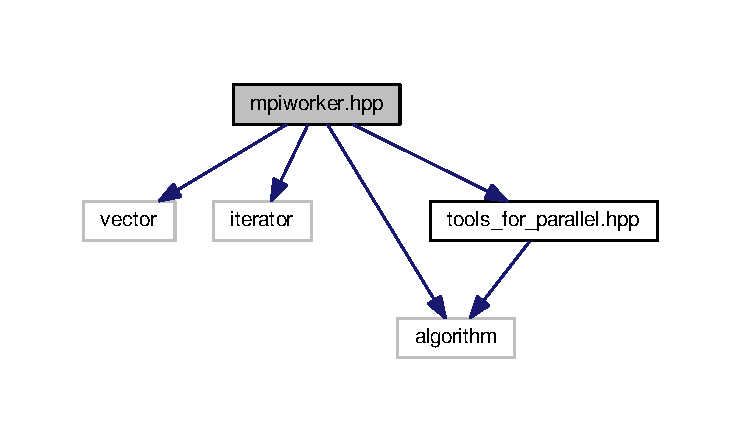
\includegraphics[width=350pt]{mpiworker_8hpp__incl}
\end{center}
\end{figure}
Граф файлов, в которые включается этот файл\-:\nopagebreak
\begin{figure}[H]
\begin{center}
\leavevmode
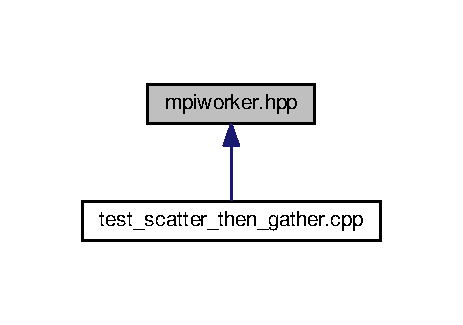
\includegraphics[width=222pt]{mpiworker_8hpp__dep__incl}
\end{center}
\end{figure}
\subsection*{Классы}
\begin{DoxyCompactItemize}
\item 
class \hyperlink{classmpiworker_1_1MPIInit}{mpiworker\-::\-M\-P\-I\-Init}
\begin{DoxyCompactList}\small\item\em Создает и удаляет коммуникатор M\-P\-I\-::\-C\-O\-M\-M\-\_\-\-W\-O\-R\-L\-D. Реализован как Singleton Meyers. Начиная с С++11 потокобезобасен \mbox{[}I\-S\-O N3337, 6.\-7.\-4\mbox{]}. \end{DoxyCompactList}\item 
class \hyperlink{classmpiworker_1_1MPIWorker}{mpiworker\-::\-M\-P\-I\-Worker}
\begin{DoxyCompactList}\small\item\em Содержит методы, выполняющие разделение и сборку массивов в M\-P\-I-\/приложении. \end{DoxyCompactList}\end{DoxyCompactItemize}
\subsection*{Пространства имен}
\begin{DoxyCompactItemize}
\item 
\hyperlink{namespacempiworker}{mpiworker}
\end{DoxyCompactItemize}

\hypertarget{test__scatter__then__gather_8cpp}{\section{test\-\_\-scatter\-\_\-then\-\_\-gather.\-cpp File Reference}
\label{test__scatter__then__gather_8cpp}\index{test\-\_\-scatter\-\_\-then\-\_\-gather.\-cpp@{test\-\_\-scatter\-\_\-then\-\_\-gather.\-cpp}}
}
{\ttfamily \#include $<$mpi.\-h$>$}\\*
{\ttfamily \#include $<$iostream$>$}\\*
{\ttfamily \#include \char`\"{}../include/mpiworker/mpiworker.\-hpp\char`\"{}}\\*
{\ttfamily \#include $<$boost/test/included/unit\-\_\-test\-\_\-framework.\-hpp$>$}\\*
Include dependency graph for test\-\_\-scatter\-\_\-then\-\_\-gather.\-cpp\-:\nopagebreak
\begin{figure}[H]
\begin{center}
\leavevmode
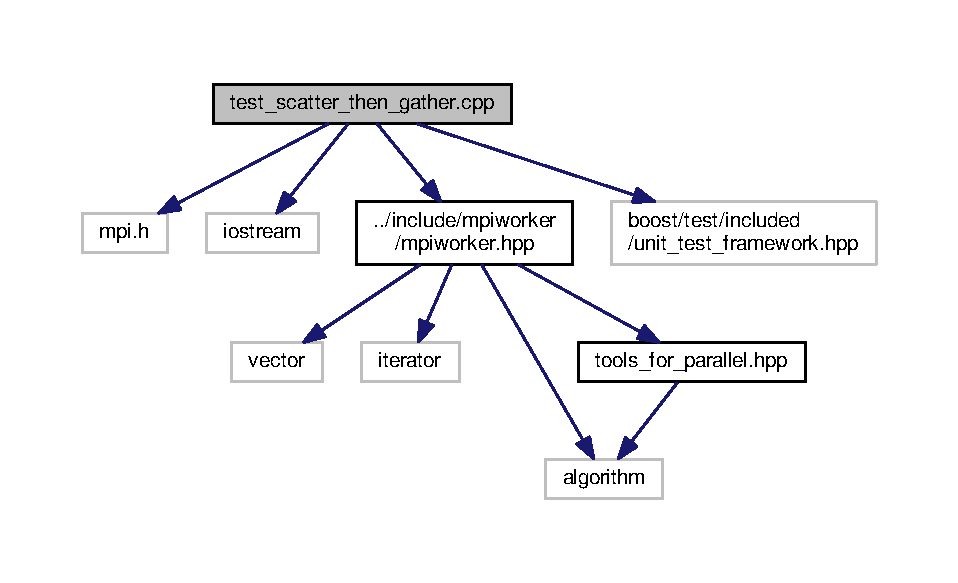
\includegraphics[width=350pt]{test__scatter__then__gather_8cpp__incl}
\end{center}
\end{figure}
\subsection*{Macros}
\begin{DoxyCompactItemize}
\item 
\#define \hyperlink{test__scatter__then__gather_8cpp_a6b2a3852db8bb19ab6909bac01859985}{B\-O\-O\-S\-T\-\_\-\-T\-E\-S\-T\-\_\-\-M\-O\-D\-U\-L\-E}~test\-\_\-scatter\-\_\-and\-\_\-gather
\end{DoxyCompactItemize}
\subsection*{Functions}
\begin{DoxyCompactItemize}
\item 
\hyperlink{test__scatter__then__gather_8cpp_a8e719c4f477459544627877df12f3a14}{B\-O\-O\-S\-T\-\_\-\-A\-U\-T\-O\-\_\-\-T\-E\-S\-T\-\_\-\-C\-A\-S\-E} (test\-\_\-scatter\-\_\-and\-\_\-gather)
\end{DoxyCompactItemize}


\subsection{Macro Definition Documentation}
\hypertarget{test__scatter__then__gather_8cpp_a6b2a3852db8bb19ab6909bac01859985}{\index{test\-\_\-scatter\-\_\-then\-\_\-gather.\-cpp@{test\-\_\-scatter\-\_\-then\-\_\-gather.\-cpp}!B\-O\-O\-S\-T\-\_\-\-T\-E\-S\-T\-\_\-\-M\-O\-D\-U\-L\-E@{B\-O\-O\-S\-T\-\_\-\-T\-E\-S\-T\-\_\-\-M\-O\-D\-U\-L\-E}}
\index{B\-O\-O\-S\-T\-\_\-\-T\-E\-S\-T\-\_\-\-M\-O\-D\-U\-L\-E@{B\-O\-O\-S\-T\-\_\-\-T\-E\-S\-T\-\_\-\-M\-O\-D\-U\-L\-E}!test_scatter_then_gather.cpp@{test\-\_\-scatter\-\_\-then\-\_\-gather.\-cpp}}
\subsubsection[{B\-O\-O\-S\-T\-\_\-\-T\-E\-S\-T\-\_\-\-M\-O\-D\-U\-L\-E}]{\setlength{\rightskip}{0pt plus 5cm}\#define B\-O\-O\-S\-T\-\_\-\-T\-E\-S\-T\-\_\-\-M\-O\-D\-U\-L\-E~test\-\_\-scatter\-\_\-and\-\_\-gather}}\label{test__scatter__then__gather_8cpp_a6b2a3852db8bb19ab6909bac01859985}


\subsection{Function Documentation}
\hypertarget{test__scatter__then__gather_8cpp_a8e719c4f477459544627877df12f3a14}{\index{test\-\_\-scatter\-\_\-then\-\_\-gather.\-cpp@{test\-\_\-scatter\-\_\-then\-\_\-gather.\-cpp}!B\-O\-O\-S\-T\-\_\-\-A\-U\-T\-O\-\_\-\-T\-E\-S\-T\-\_\-\-C\-A\-S\-E@{B\-O\-O\-S\-T\-\_\-\-A\-U\-T\-O\-\_\-\-T\-E\-S\-T\-\_\-\-C\-A\-S\-E}}
\index{B\-O\-O\-S\-T\-\_\-\-A\-U\-T\-O\-\_\-\-T\-E\-S\-T\-\_\-\-C\-A\-S\-E@{B\-O\-O\-S\-T\-\_\-\-A\-U\-T\-O\-\_\-\-T\-E\-S\-T\-\_\-\-C\-A\-S\-E}!test_scatter_then_gather.cpp@{test\-\_\-scatter\-\_\-then\-\_\-gather.\-cpp}}
\subsubsection[{B\-O\-O\-S\-T\-\_\-\-A\-U\-T\-O\-\_\-\-T\-E\-S\-T\-\_\-\-C\-A\-S\-E}]{\setlength{\rightskip}{0pt plus 5cm}B\-O\-O\-S\-T\-\_\-\-A\-U\-T\-O\-\_\-\-T\-E\-S\-T\-\_\-\-C\-A\-S\-E (
\begin{DoxyParamCaption}
\item[{test\-\_\-scatter\-\_\-and\-\_\-gather}]{}
\end{DoxyParamCaption}
)}}\label{test__scatter__then__gather_8cpp_a8e719c4f477459544627877df12f3a14}
Выполняется тестирование операторов scattrv и gatherv. Для сборки только этого теста выполните команду
\begin{DoxyCode}
make test\_scatter\_then\_gather 
\end{DoxyCode}
 и запустите его на исполнение, например
\begin{DoxyCode}
mpirun -np 2 ./test\_scatter\_then\_gather 
\end{DoxyCode}
 
\hypertarget{tools__for__parallel_8hpp}{\section{tools\-\_\-for\-\_\-parallel.\-hpp File Reference}
\label{tools__for__parallel_8hpp}\index{tools\-\_\-for\-\_\-parallel.\-hpp@{tools\-\_\-for\-\_\-parallel.\-hpp}}
}
{\ttfamily \#include $<$algorithm$>$}\\*
Include dependency graph for tools\-\_\-for\-\_\-parallel.\-hpp\-:\nopagebreak
\begin{figure}[H]
\begin{center}
\leavevmode
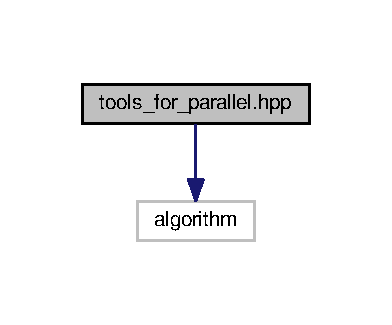
\includegraphics[width=188pt]{tools__for__parallel_8hpp__incl}
\end{center}
\end{figure}
This graph shows which files directly or indirectly include this file\-:\nopagebreak
\begin{figure}[H]
\begin{center}
\leavevmode
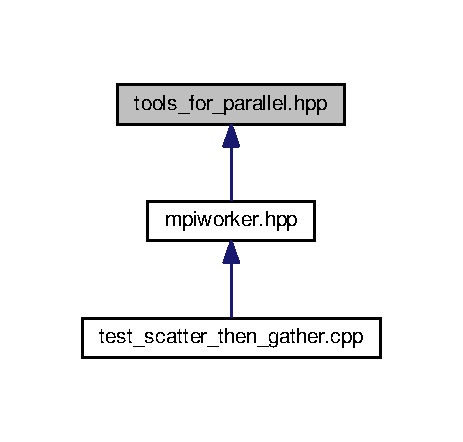
\includegraphics[width=222pt]{tools__for__parallel_8hpp__dep__incl}
\end{center}
\end{figure}
\subsection*{Functions}
\begin{DoxyCompactItemize}
\item 
{\footnotesize template$<$typename Iterator , typename Size\-Type $>$ }\\void \hyperlink{group__MPIWorker_ga6fd8303c1b4e39a4a623756fdcbeae6f}{calculate\-Portions} (Size\-Type n\-Elems, Iterator beg\-Counts, Iterator end\-Counts, Iterator beg\-Displs, Iterator end\-Displs, bool is\-Zero\-Work=false)
\end{DoxyCompactItemize}

%--- End generated contents ---

% Index
\newpage
\phantomsection
\addcontentsline{toc}{chapter}{Алфавитный указатель}
\printindex

\end{document}
